En este apartado se presentan los resultados obtenidos en la realización de un
estudio cuantitativo sobre la literatura científica de los últimos años. Dichos
resultados no se analizarán en profundidad, conteniendo este apartado únicamente,
una descripción de los mismos.

En este estudio se han clasificado multitud de textos referentes a la
sostenibilidad, para analizar si existe algún patrón u objetivo predominante en
este ámbito de estudio. 

Como primer paso se han extraído un total de 100.000 textos de \textit{Scopus},
una de las principales bases de datos académicas. Estos textos están divididos
de manera equitativa entre los años 2019 y 2023, contando con 20.000 de cada
año. Este número es debido a que esta es la cantidad máxima que la plataforma
permite exportar. Seguramente esta limitación pueda ser abordad de alguna
manera, pudiendo obtener todas las publicaciones de cada año. Esto se consideró
en un principio, pero más tarde se llegó a al conclusión de que 20.000 era una
población suficiente de datos como para poder identificar, si existe, algún
patrón en las publicaciones. Adicionalmente el rango de años elegido ha sido de 5 años ya que se considera que este es suficiente para poder, por un lado,obtener una métricas relevantes en cuanto al esfuerzo investigador realizado en cada objetivo y por otro poder identificar alguna tendencia en los datos, teniendo en cuenta el impacto que la pandemia de COVID19 ha tenido en la sociedad.

Estos textos fueron clasificados usando el modelo que mejor resultados obtuvo en
las validaciones, siendo este el 23. Los resultados obtenidos se encuentran a
continuación representados en la tabla \cref{table:Datos resultantes del estudio}

\begin{table}[H]
    \begin{tabular}{|c || c | c | c | c | c | c |}
        \hline
        ODS/Año & 2019 & 2020 & 2021 & 2022 & 2023 & Total \\ \hline
                                                              \hline
        ODS1  & 163  & 160  & 180  & 155  & 170    & 828   \\ \hline
        ODS2  & 2063 & 2273 & 2498 & 2354 & 2304   & 11492 \\ \hline
        ODS3  & 1742 & 1859 & 2002 & 2057 & 1884   & 9544  \\ \hline
        ODS4  & 511  & 535  & 459  & 472  & 386    & 2363  \\ \hline
        ODS5  & 256  & 255  & 261  & 243  & 221    & 1236  \\ \hline
        ODS6  & 1012 & 1068 & 1062 & 980  & 984    & 5106  \\ \hline
        ODS7  & 1777 & 1730 & 1885 & 1900 & 2021   & 9313  \\ \hline
        ODS8  & 908  & 874  & 880  & 927  & 884    & 4473  \\ \hline
        ODS9  & 2031 & 1960 & 1964 & 2219 & 2447   & 10621 \\ \hline
        ODS10 & 109  & 103  & 83   & 91   & 94     & 480   \\ \hline
        ODS11 & 2099 & 1922 & 1776 & 1684 & 1616   & 9097  \\ \hline
        ODS12 & 4405 & 4550 & 4605 & 5012 & 5361   & 23933 \\ \hline
        ODS13 & 1304 & 1311 & 1486 & 1633 & 1767   & 7501  \\ \hline
        ODS14 & 801  & 816  & 887  & 755  & 738    & 3997  \\ \hline
        ODS15 & 2337 & 2300 & 2303 & 2198 & 2078   & 11216 \\ \hline
        ODS16 & 161  & 166  & 145  & 115  & 128    & 715   \\ \hline
        ODS17 & 1829 & 1765 & 1641 & 1702 & 1688   & 8625  \\ \hline
    \end{tabular}
    \caption{Datos resultantes del estudio}
    \label{table:Datos resultantes del estudio}
\end{table}


Esta tabla, \cref{table:Datos resultantes del estudio}, contiene los datos de
manera condensada pero su interpretación puede ser complicada, es por esto por
lo que se presentarán diversas representaciones de los datos en forma de
gráficas para su fácil interpretación.

\section{Análisis de resultados generales}
Como primera representación de los resultados se incluye la gráfica,
\cref{fig:Resultados generales}, la cual contiene el número total de textos
clasificados por objetivo, entre los años 2019 y 2023. En esta se puede apreciar
de manera más notable que el objetivo con más textos relacionados es el 12,
seguido de una serie de objetivos con una relevancia similar, los 2, 3, 7, 9,
11, 13, 15 y 17. Estos tienen un número de publicaciones similares. Destacan
también los objetivos 1, 10 y 16 por el número tan bajo de publicaciones
relacionadas.

\begin{figure}[H]
    \centering
    \includegraphics[scale=0.75]{imagenes/metricas\_totales\_generales.eps}
    \captionsetup{justification=centering}
    \caption{Resultados generales}
    \label{fig:Resultados generales}
\end{figure}

\section{Evolución de publicaciones}
A continuación se muestra la evolución en el número de publicaciones de los objetivos más relevantes a lo largo de los años. La evolución del resto se encontrará al final del apartado de una manera más compacta, de esta manera se pueden apreciar las tendencias de estos objetivos. 

\subsubsection{Objetivo 12}
Este primer objetivo es el más relevante en cuanto al número de publicaciones, duplicando en magnitud a los objetivos siguientes. En la \cref{fig:Evolución ODS 12} se puede apreciar la tendencia en  el número de publicaciones de este objetivo y como  esta va en aumento cada año, haciendo esto de una manera lineal y más o menos constante ya que cada año tiene más investigaciones que el anterior. 
\begin{figure}[H]
    \centering
    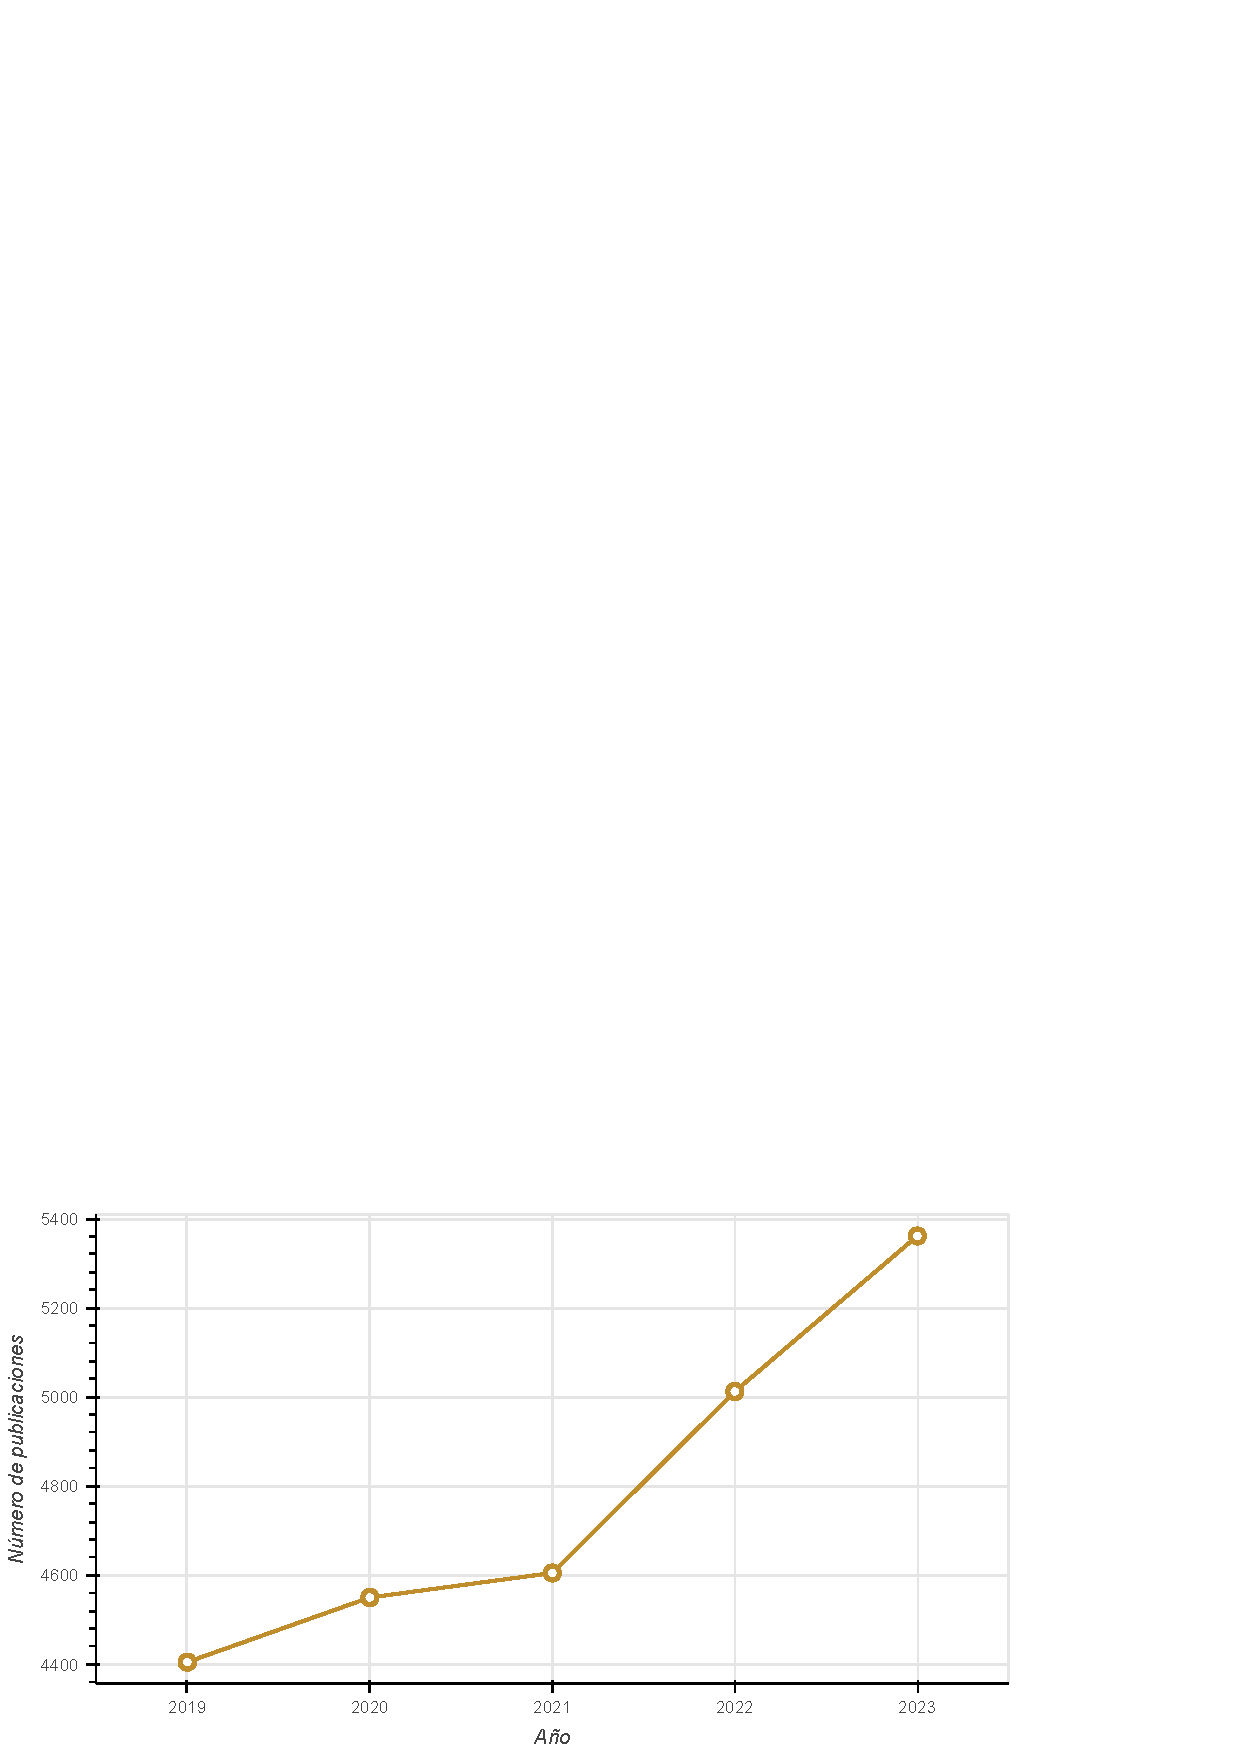
\includegraphics[scale=0.75]{EvolucionOds12}
    \captionsetup{justification=centering}
    \caption{Evolución ODS 12}
    \label{fig:Evolución ODS 12}
\end{figure}

\subsubsection{Objetivo 3}
Aunque no tan relevante en cuanto a métricas, el objetivo 3 tiene una relevancia especial debido a la pandemia generada por el coronavirus. El impacto que esta tuvo en la sociedad debería verse reflejado en un aumento en el número de publicaciones relacionadas con el objetivo 3. Esta correlación se ve reflejada en la \cref{fig:Evolución ODS 3}, teniendo esta una tendencia ascendente y más acelerada que el objetivo 12 durante los años posteriores a 2019 pero esta se ve frenada de manera contundente en 2023. Aunque exista esta correlación solo con estos datos no se puede llegar a conclusiones en cuanto a causalidad pero la posibilidad tampoco se puede negar.

\begin{figure}[H]
    \centering
    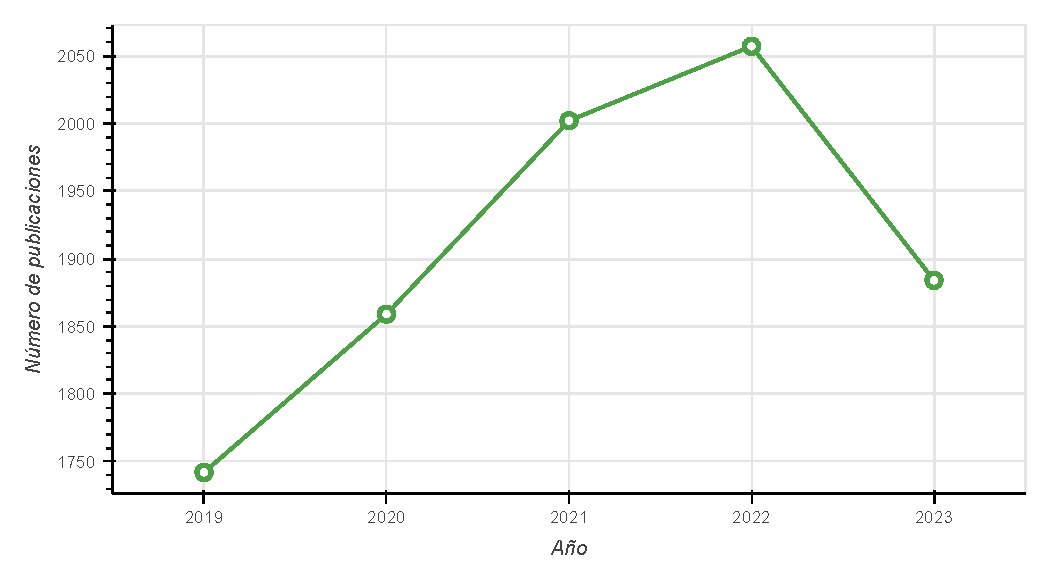
\includegraphics[scale=0.75]{EvolucionOds3}
    \captionsetup{justification=centering}
    \caption{Evolución ODS 3}
    \label{fig:Evolución ODS 3}
\end{figure}

\subsubsection{Objetivo 9}
La relevancia de este objetivo es constante, ya que la industria es uno de los principales motores económicos y de desarrollo humano, estando en los últimos años en la vanguardia tecnológica con el auge de la industria 4.0. Esta tendencia se ve reflejada en la gráfica, \cref{fig:Evolución ODS 9}, estando el número de publicaciones relativamente estancado, aunque con un número alto de ellas, durante los años entre 2019 y 2021 y sufriendo un auge repentino a partir de 2022, manteniéndose esta tendencia a lo largo de 2023.
\begin{figure}[H]
    \centering
    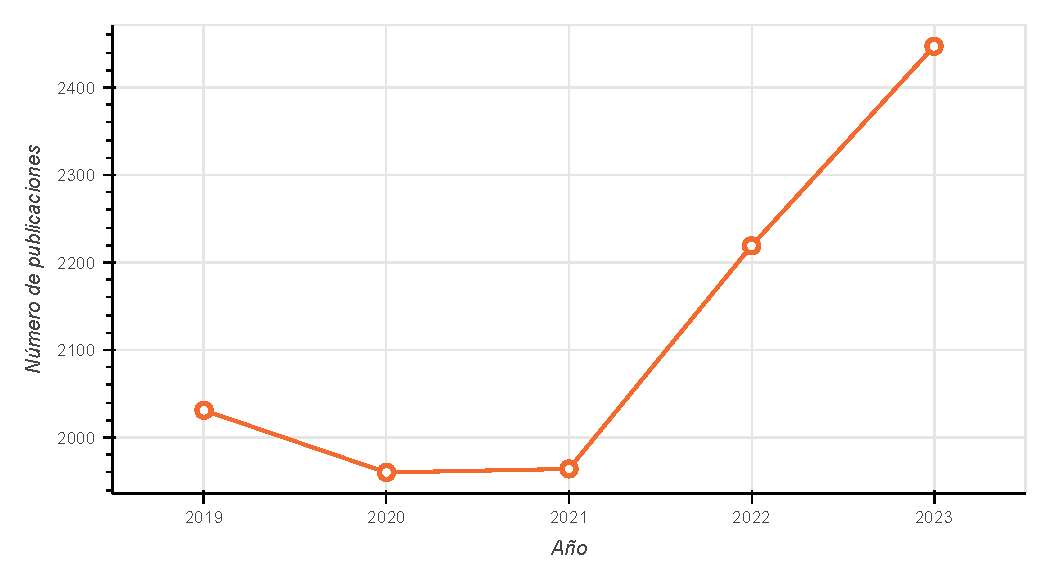
\includegraphics[scale=0.75]{EvolucionOds9}
    \captionsetup{justification=centering}
    \caption{Evolución ODS 9}
    \label{fig:Evolución ODS 9}
\end{figure}

\subsubsection{Objetivo 2}
La importancia de este objetivo en el contexto estudiado recae en su segundo lugar como objetivo con mayor número de publicaciones relacionadas, siendo estas, como se aprecia con mayor claridad en la tabla \cref{table:Datos resultantes del estudio}, de 11.492. Aún siendo la mitad que los obtenidos por el objetivo 12, es un número cuanto menos relevante. En la \cref{fig:Evolución ODS 2} se puede observar una tendencia ascendente desde 2019, con un pico en 2021 y una posterior tendencia descendiente hasta 2023.
\begin{figure}[H]
    \centering
    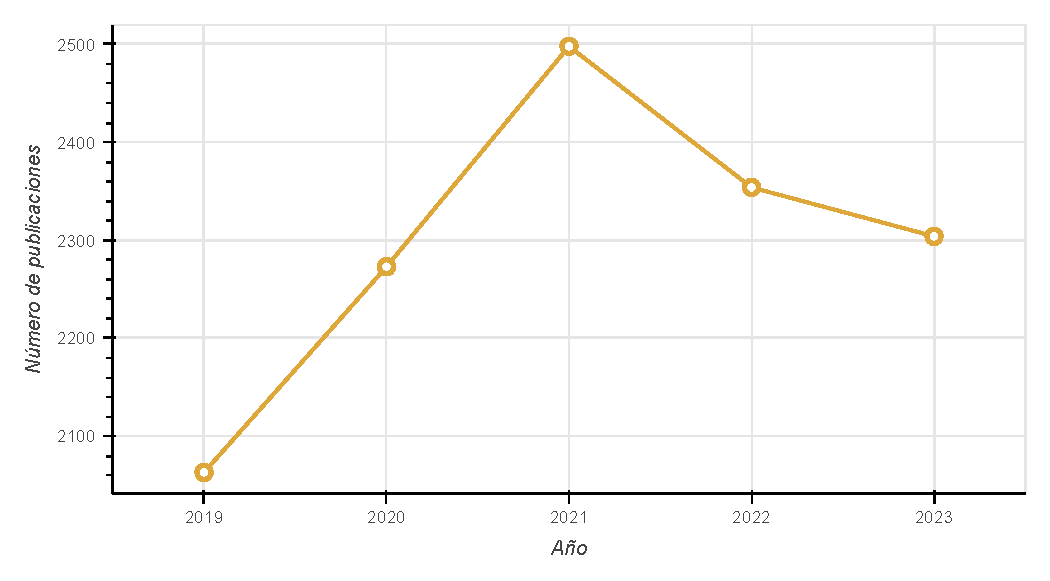
\includegraphics[scale=0.75]{EvolucionOds2}
    \captionsetup{justification=centering}
    \caption{Evolución ODS 2}
    \label{fig:Evolución ODS 2}
\end{figure}

\subsubsection{Objetivo 15}
Finalmente se incluye el objetivo 15 como último objetivo relevante, siendo este el tercero con más publicaciones relacionadas, por detrás del 2. Este, de todos los objetivos analizados, tiene la única gráfica que muestra una tendencia general descendiente, \cref{fig:Evolucion ODS 15}, con la notable excepción de las publicaciones de 2021, siendo estas ligeramente superiores a las de 2020. Resalta sobre todo la tendencia descendiente tan drástica vista justo después de este aumento en publicaciones. 
\begin{figure}[H]
    \centering
    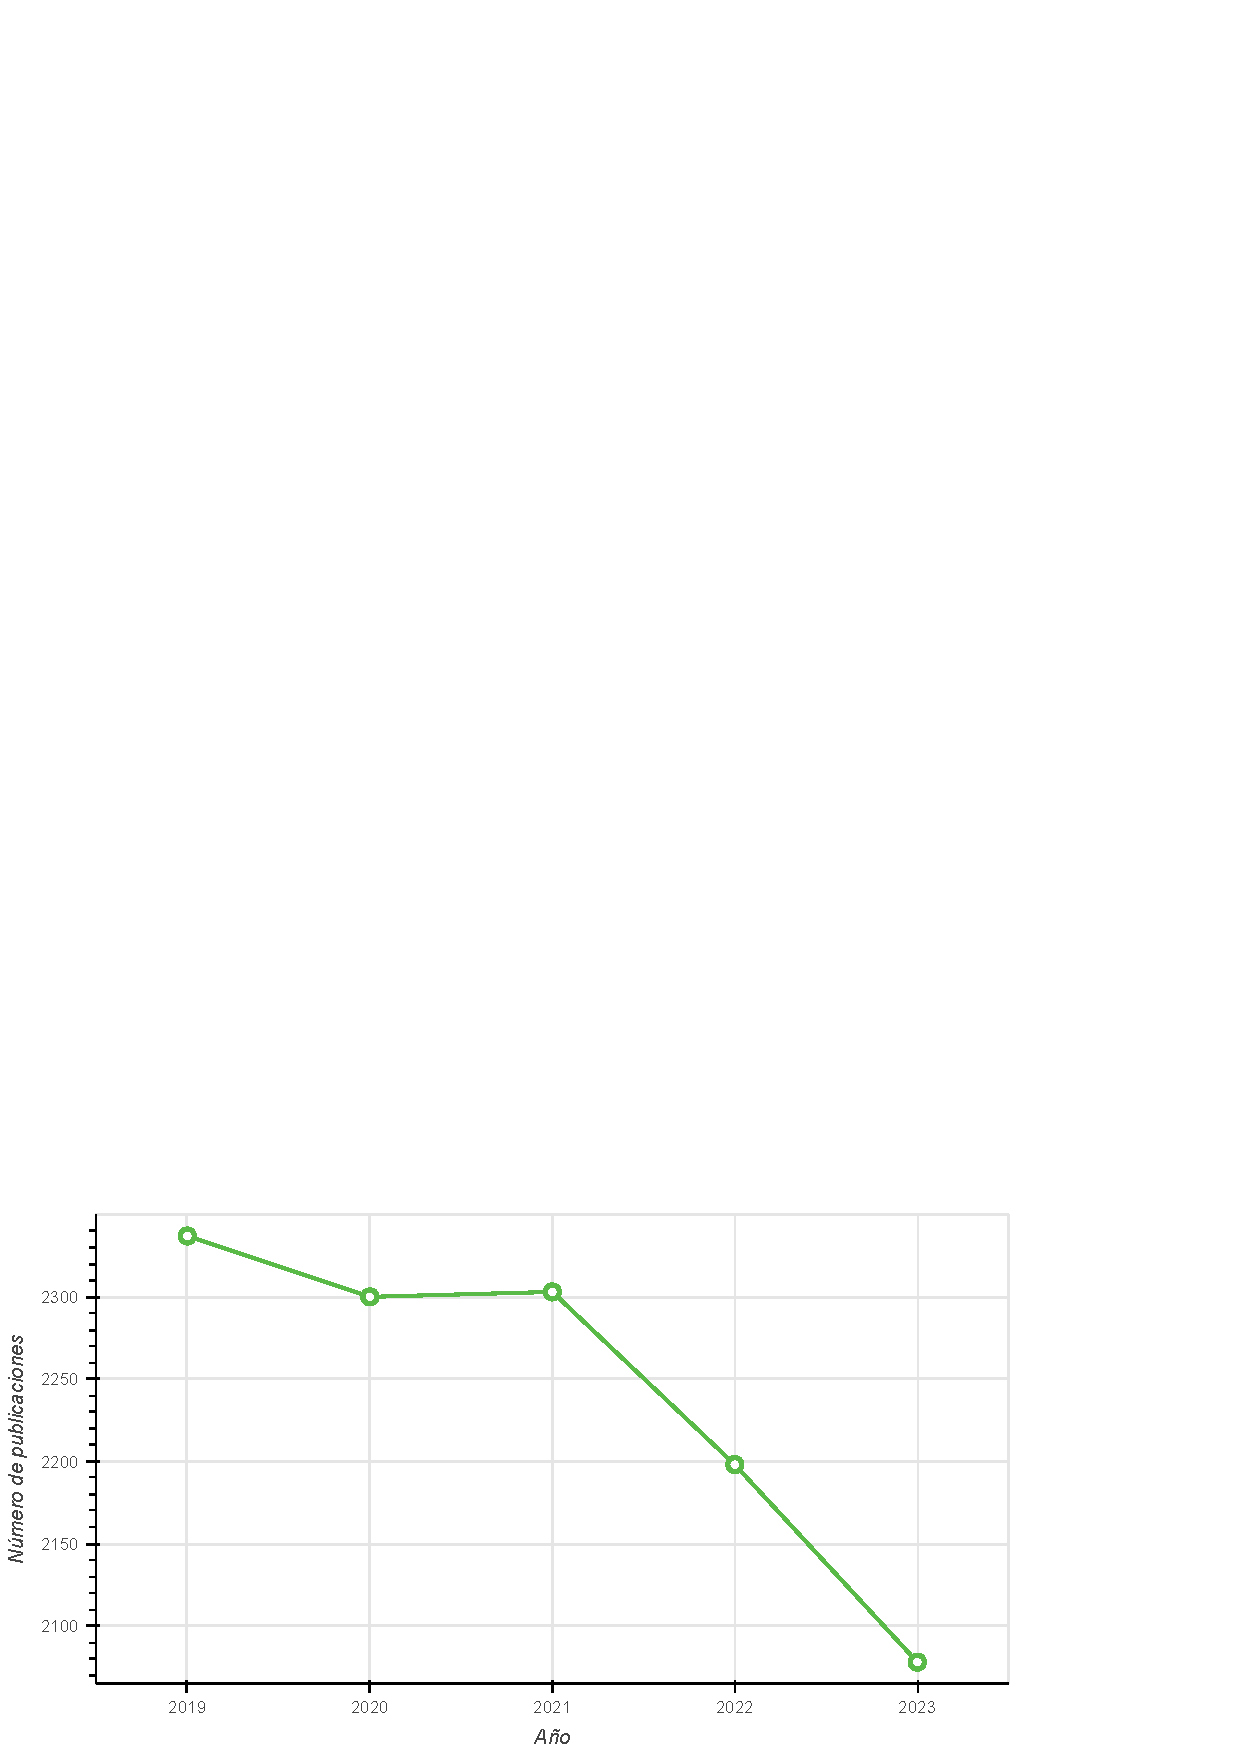
\includegraphics[scale=0.75]{EvolucionOds15}
    \captionsetup{justification=centering}
    \caption{Evolución ODS 15}
    \label{fig:Evolucion ODS 15}
\end{figure}

\subsubsection{Objetivos adicionales}
A continuación se muestran las gráficas de tendencias del resto de objetivs, \cref{fig:Resto de tendencias}, considerados menos relevantes como para mencionar y, por motivos de espacio y claridad, se incluirán en dos columnas. De esta manera las tendencias serán fácilmente distinguibles, pudiendo consultar los número en la tabla \cref{table:Datos resultantes del estudio}. Dentro de estas se ven multitud de  tendencias diferentes, no pudiendo identificar ningún patrón común entre ellas. Destacar adicionalmente la gráfica referente al objetivo 11, \cref{fig:Evolucion ods11}, siendo este uno de los objetivos con mayor número de publicaciones y contando con  una tendencia descendente desde 2019.

\begin{figure}[H]
    \begin{subfigure}{0.45\textwidth}
        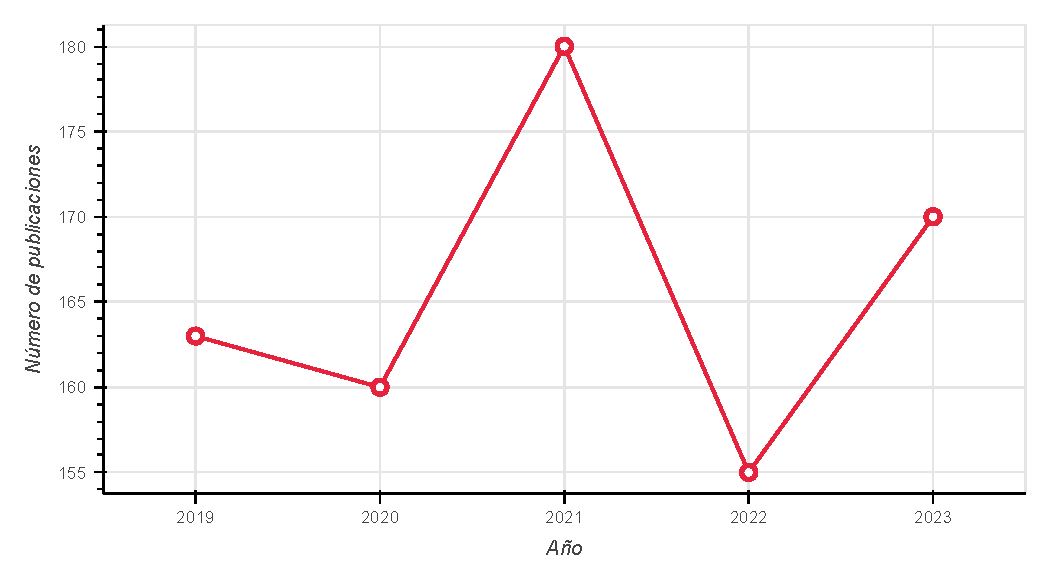
\includegraphics[width=0.9\linewidth]{imagenes/EvolucionOds1.eps} 
        \captionsetup{justification=centering}
        \caption{Evolucion ODS1}
        \label{fig:Evolucion ods1}
    \end{subfigure}
    \begin{subfigure}{0.45\textwidth}
        \includegraphics[width=0.9\linewidth]{imagenes/EvolucionOds4.eps} 
        \captionsetup{justification=centering}
        \caption{Evolucion ODS4}
        \label{fig:Evolucion ods4}
    \end{subfigure}
        \begin{subfigure}{0.45\textwidth}
        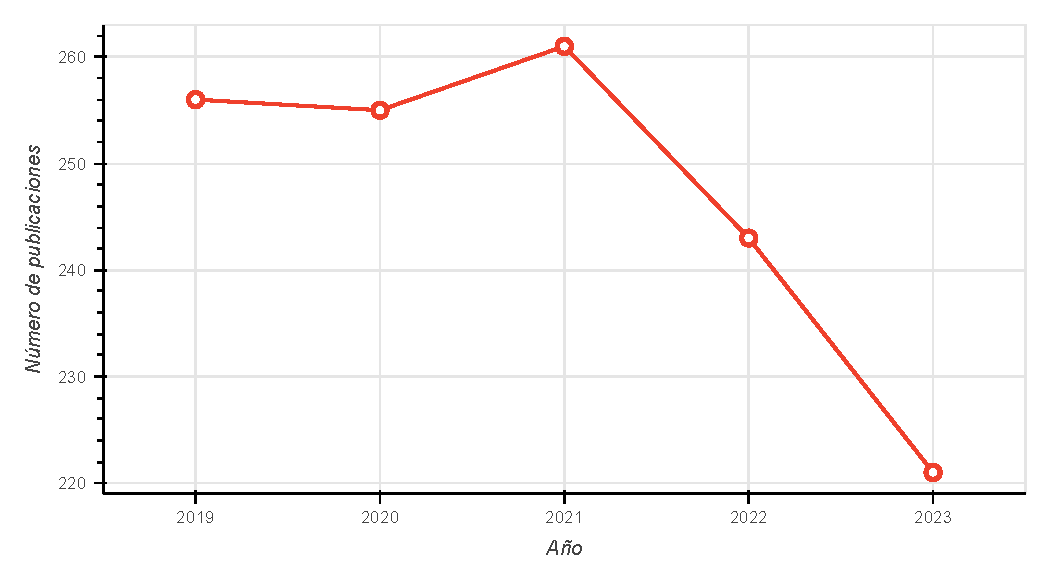
\includegraphics[width=0.9\linewidth]{imagenes/EvolucionOds5.eps} 
        \captionsetup{justification=centering}
        \caption{Evolucion ODS5}
        \label{fig:Evolucion ods5}
    \end{subfigure}
    \begin{subfigure}{0.45\textwidth}
        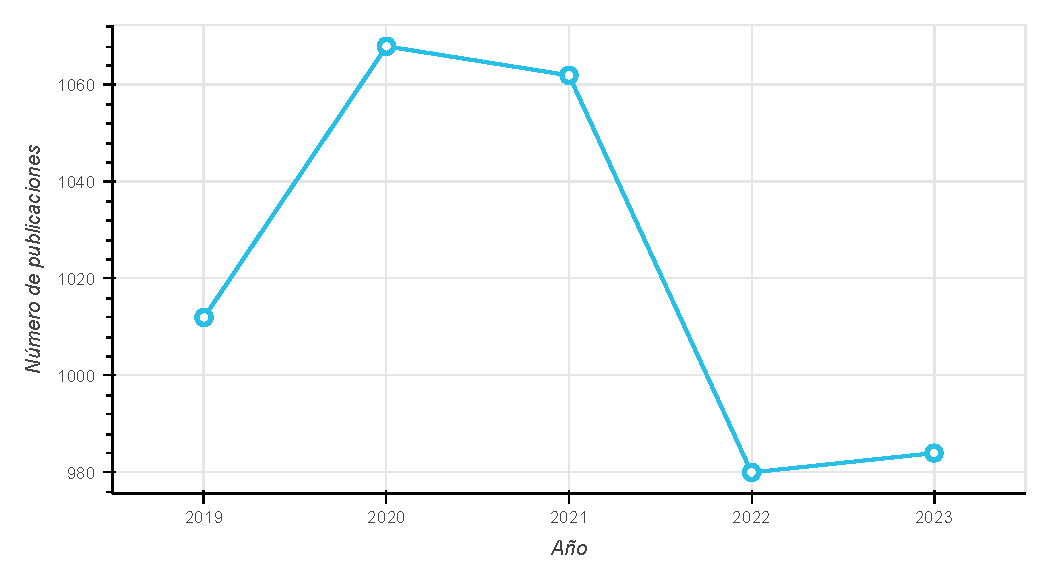
\includegraphics[width=0.9\linewidth]{imagenes/EvolucionOds6.eps} 
        \captionsetup{justification=centering}
        \caption{Evolucion ODS6}
        \label{fig:Evolucion ods6}
    \end{subfigure}
    \begin{subfigure}{0.45\textwidth}
        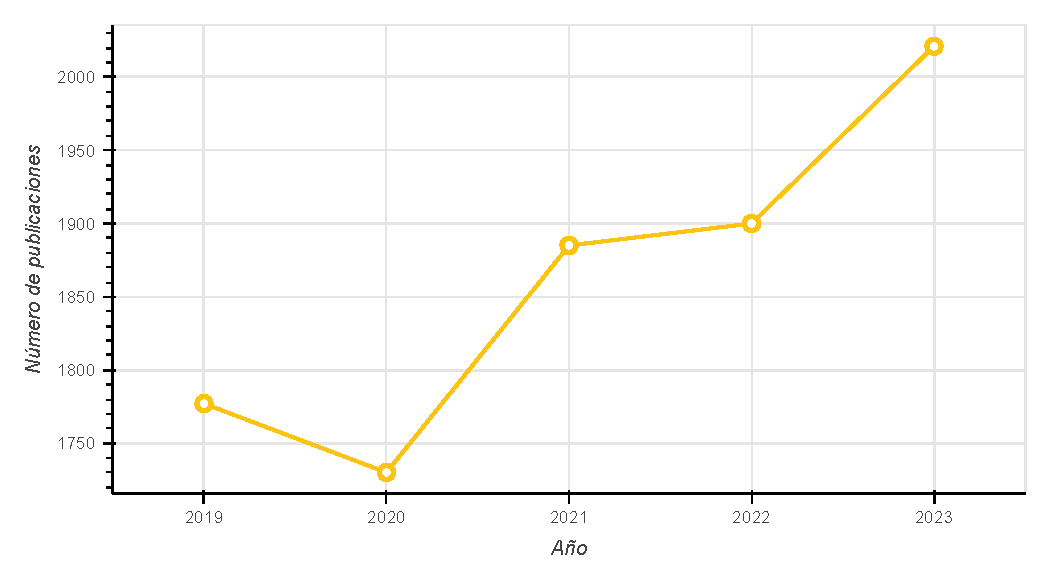
\includegraphics[width=0.9\linewidth]{imagenes/EvolucionOds7.eps} 
        \captionsetup{justification=centering}
        \caption{Evolucion ODS7}
        \label{fig:Evolucion ods7}
    \end{subfigure}
    \begin{subfigure}{0.45\textwidth}
        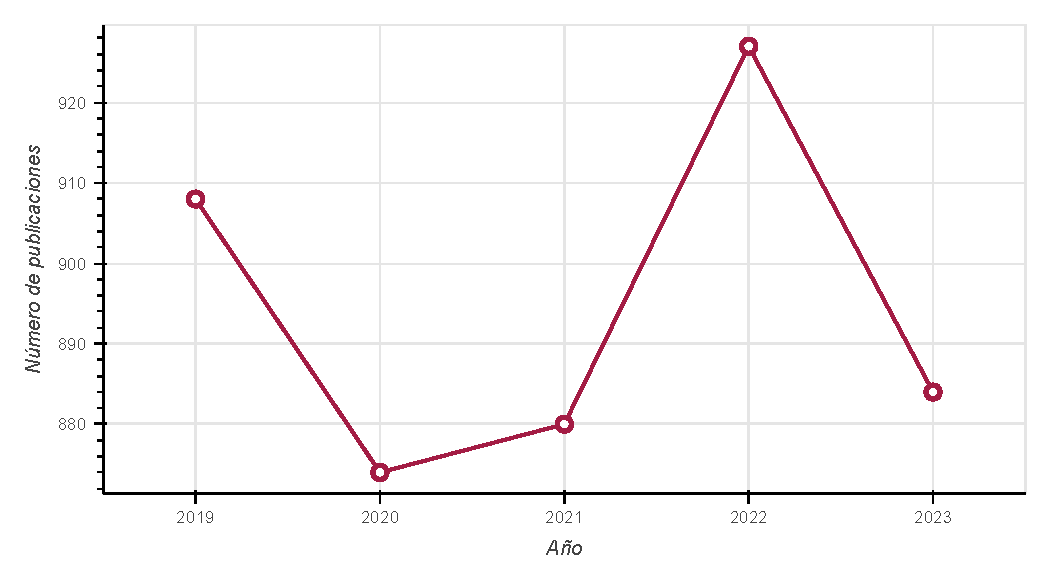
\includegraphics[width=0.9\linewidth]{imagenes/EvolucionOds8.eps} 
        \captionsetup{justification=centering}
        \caption{Evolucion ODS8}
        \label{fig:Evolucion ods8}
    \end{subfigure}
    \begin{subfigure}{0.45\textwidth}
        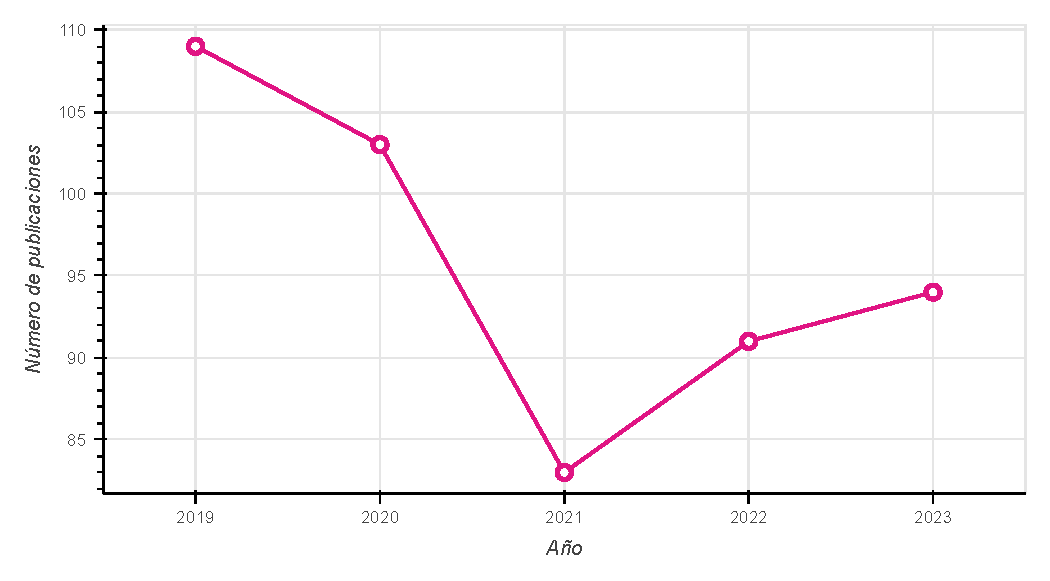
\includegraphics[width=0.9\linewidth]{imagenes/EvolucionOds10.eps} 
        \captionsetup{justification=centering}
        \caption{Evolucion ODS10}
        \label{fig:Evolucion ods10}
    \end{subfigure}
    \begin{subfigure}{0.45\textwidth}
        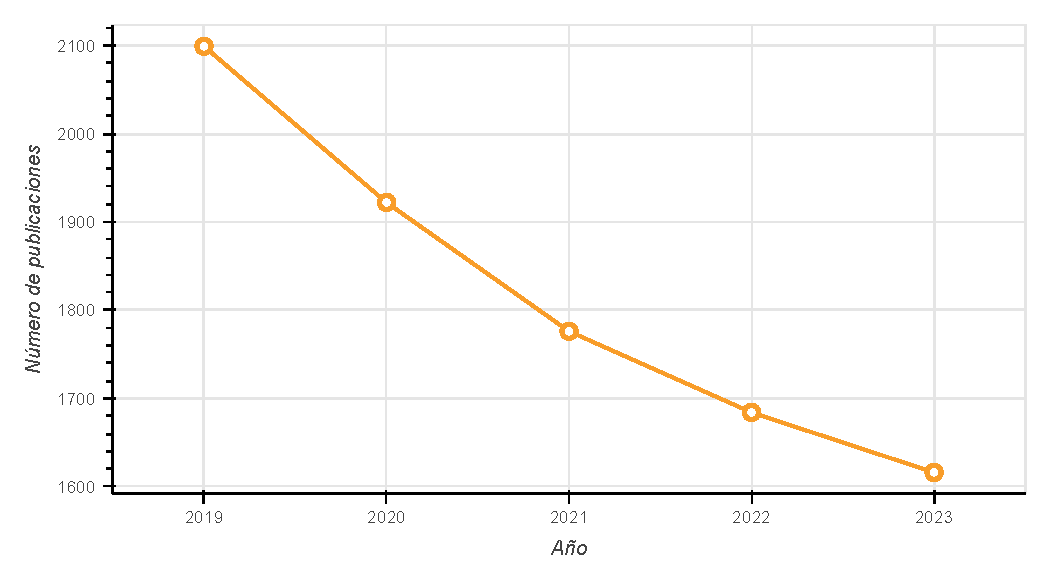
\includegraphics[width=0.9\linewidth]{imagenes/EvolucionOds11.eps} 
        \captionsetup{justification=centering}
        \caption{Evolucion ODS11}
        \label{fig:Evolucion ods11}
    \end{subfigure}
    \begin{subfigure}{0.45\textwidth}
        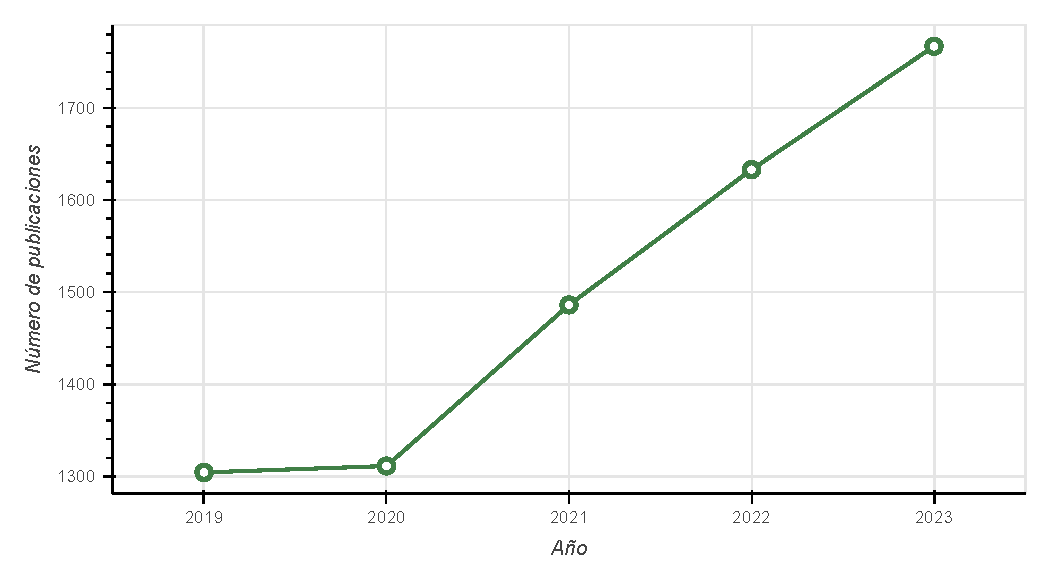
\includegraphics[width=0.9\linewidth]{imagenes/EvolucionOds13.eps} 
        \captionsetup{justification=centering}
        \caption{Evolucion ODS13}
        \label{fig:Evolucion ods13}
    \end{subfigure}
    \begin{subfigure}{0.45\textwidth}
        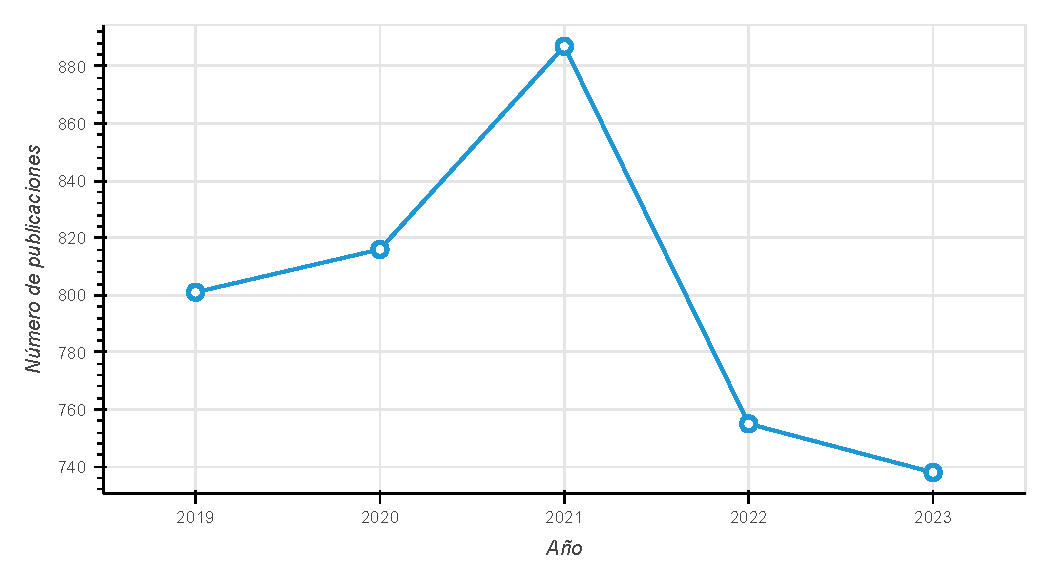
\includegraphics[width=0.9\linewidth]{imagenes/EvolucionOds14.eps} 
        \captionsetup{justification=centering}
        \caption{Evolucion ODS14}
        \label{fig:Evolucion ods14}
    \end{subfigure}
    \begin{subfigure}{0.45\textwidth}
        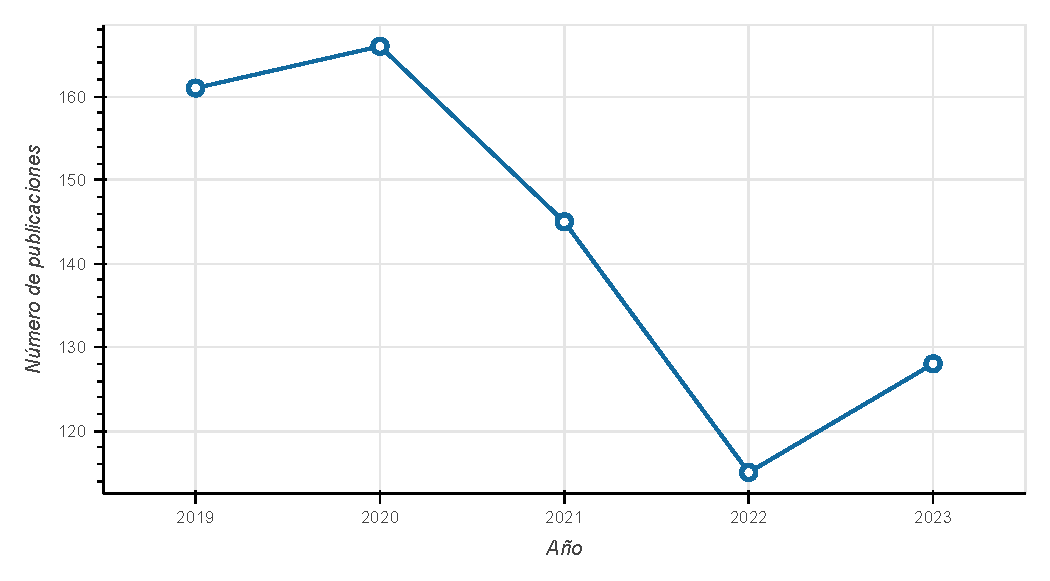
\includegraphics[width=0.9\linewidth]{imagenes/EvolucionOds16.eps} 
        \captionsetup{justification=centering}
        \caption{Evolucion ODS16}
        \label{fig:Evolucion ods16}
    \end{subfigure}
    \begin{subfigure}{0.45\textwidth}
        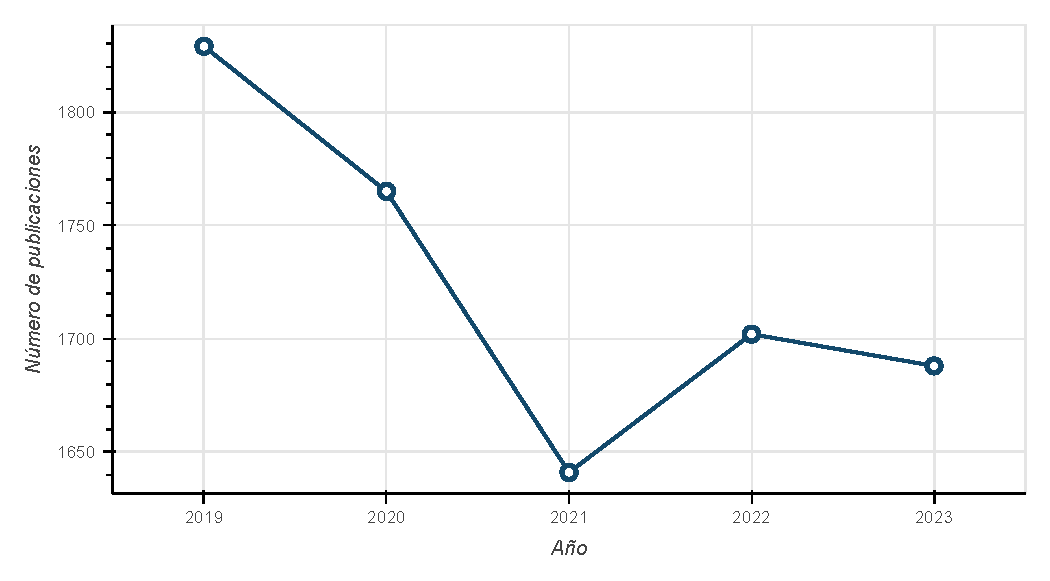
\includegraphics[width=0.9\linewidth]{imagenes/EvolucionOds17.eps} 
        \captionsetup{justification=centering}
        \caption{Evolucion ODS17}
        \label{fig:Evolucion ods17}
    \end{subfigure}
        \captionsetup{justification=centering}
    \caption{Evolución del resto de objetivos}
    \label{fig:Resto de tendencias}
\end{figure}

\section{Proporciones generales}

Como última representación de los datos se incluye, en la \cref{fig:Relaciones generales ODSs}, un gráfico en forma de anillo en el que se muestran la proporción del número de clasificaciones de todos los objetivos en el conjunto general de datos. Este gráfico, representado en un formato inspirado en  el logo original de los \gls{ODSa}, muestra las verdaderas relaciones de estos, dentro del contexto científico.

\begin{figure}[H]
    \centering
    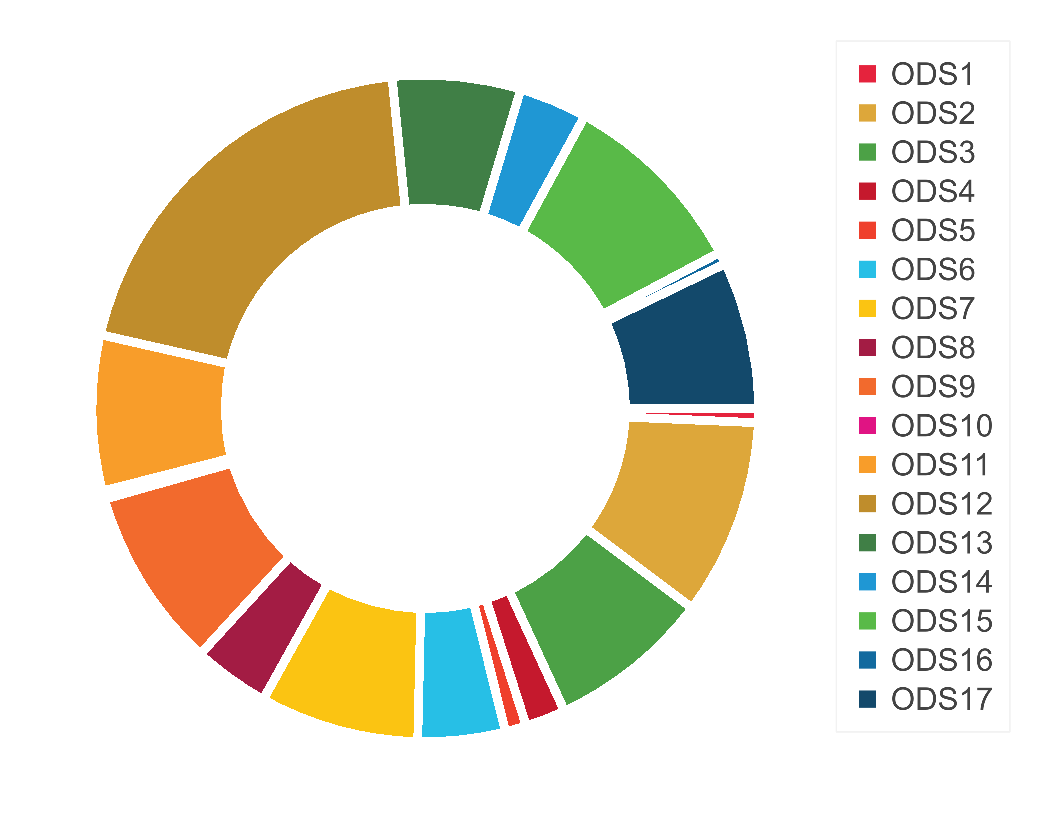
\includegraphics[scale=0.6]{imagenes/resultados_queso.eps}
    \captionsetup{justification=centering}
    \caption{Porcentaje de artículos por ODSa}
    \label{fig:Relaciones generales ODSs}
\end{figure}
